\section{测试、运行情况}

\subsection{蜗壳大雾实验工具}

本程序的每一个实验模块由组员完成后,组长会进行代码审核与测试,
如果发现问题则要求继续修改,直到所有问题被解决后该实验模块才会发布。
我们还建立了用户 QQ 群,并即时反馈用户提出的任何问题。

另一方面,各种 API 的编写与模块化编程也让我们的程序在编写过程中更不容易出错,
同时规范、统一的码风也让调试变得轻松。

% \begin{figure}[htbp]
%   \centering
%   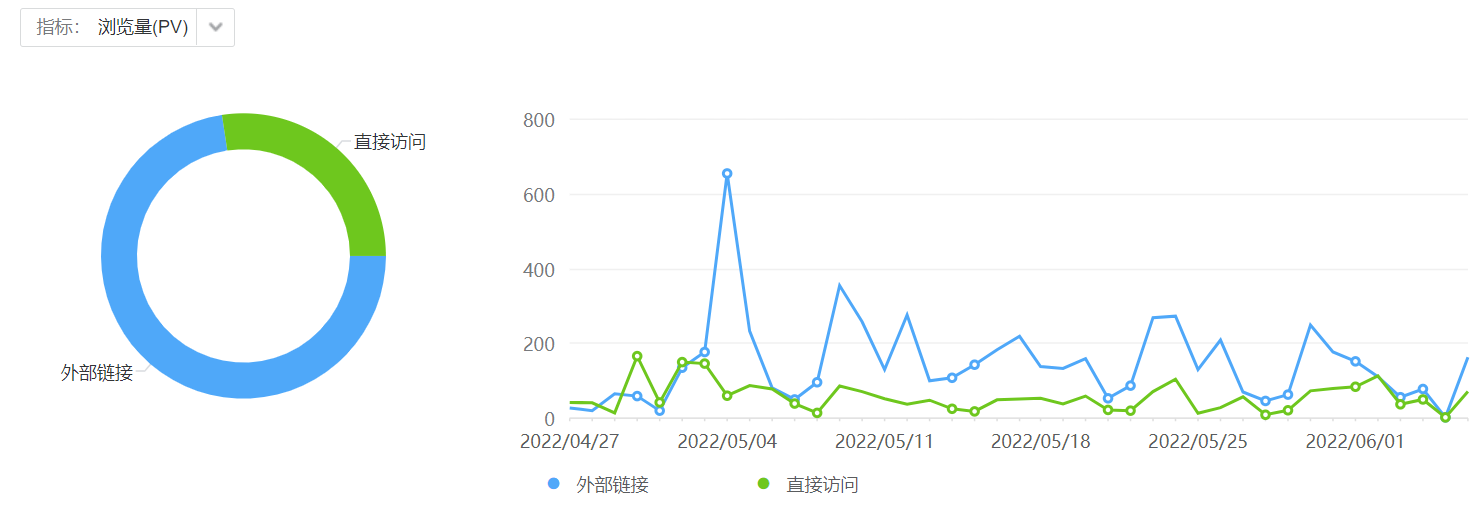
\includegraphics[width=\columnwidth]{figure/0.png}
%   \caption{4 月 27 日至 6 月 7 日的网站浏览量}
%   \label{fig:0}
% \end{figure}
% \begin{figure}[htbp]
%   \centering
%   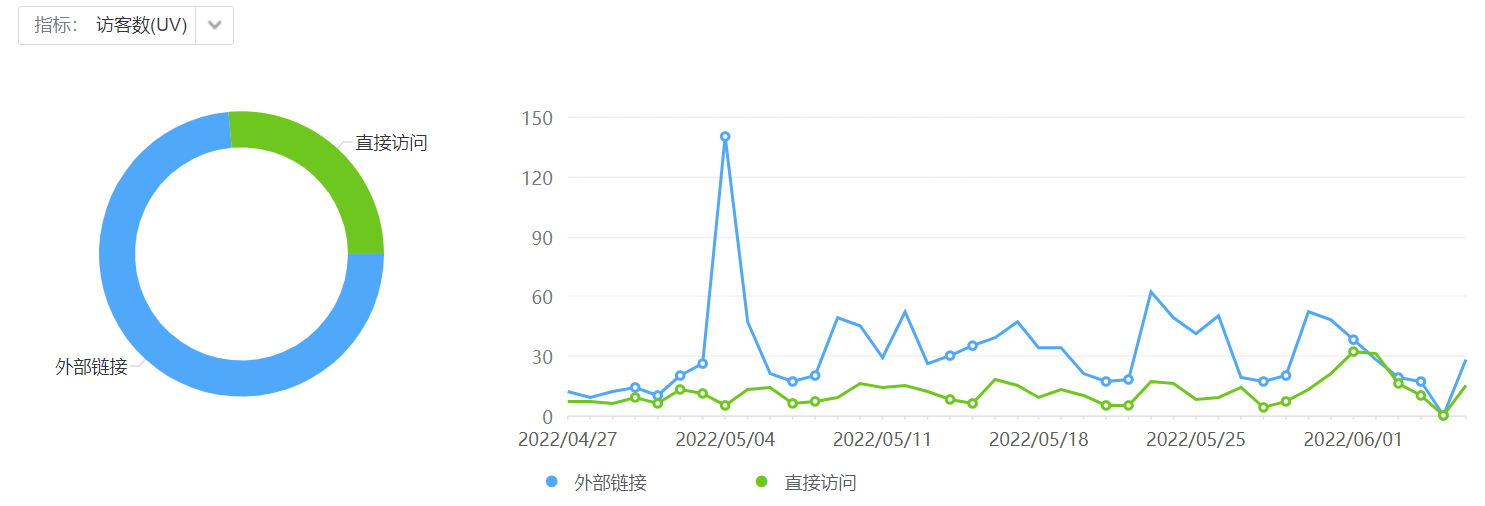
\includegraphics[width=\columnwidth]{figure/1.png}
%   \caption{4 月 27 日至 6 月 7 日的网站访客数}
%   \label{fig:1}
% \end{figure}

工具网站的访问统计如图 \ref{fig:2} 所示,可以看出我们的工具有 1000 名稳定用户。
同时,本工具在 GitHub 上开源,同学们可以进一步完善其功能。

\begin{figure}[htbp]
  \centering
  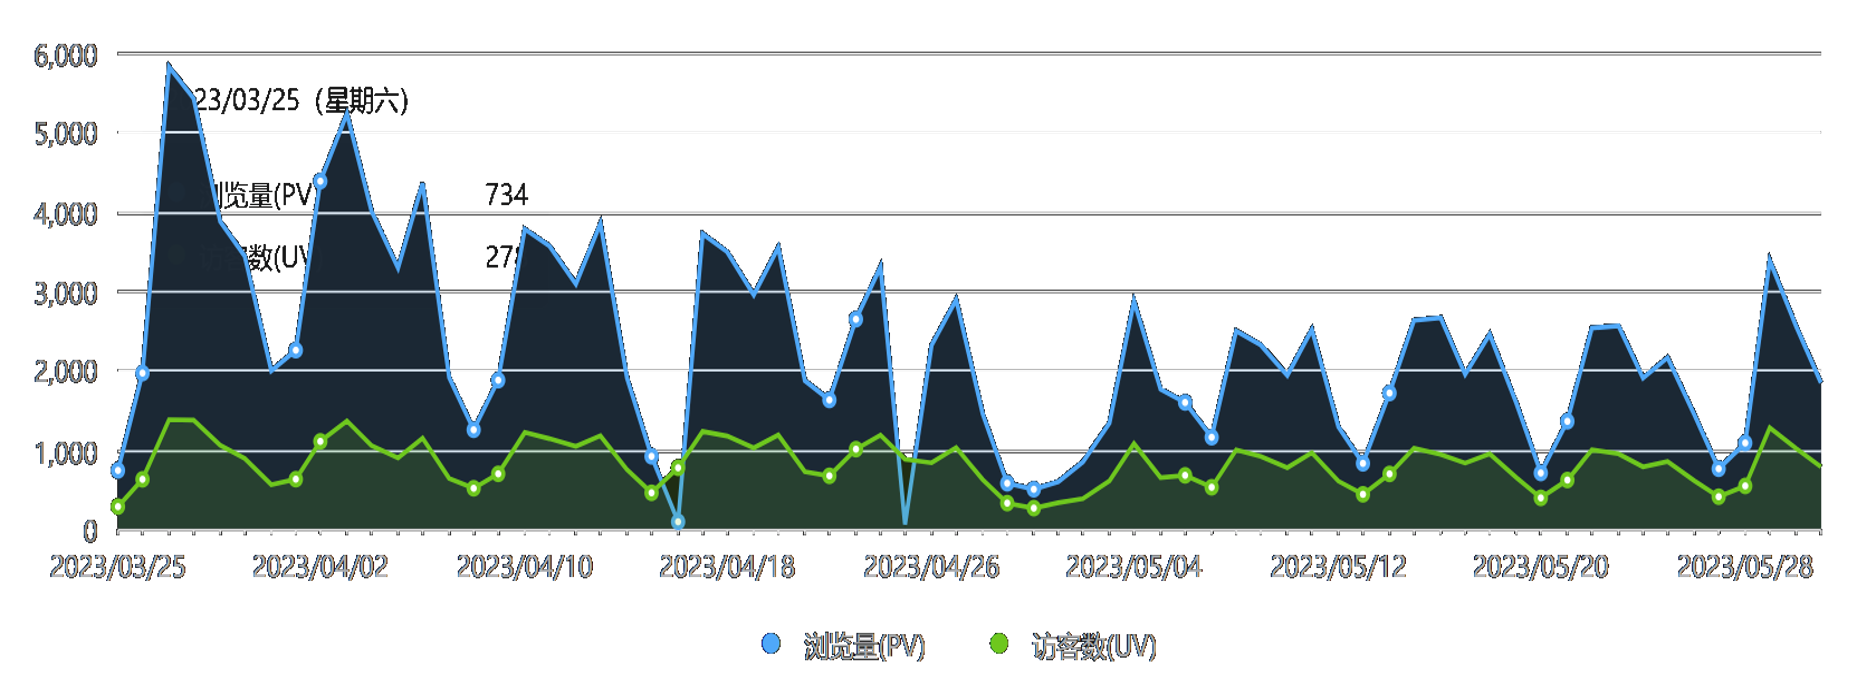
\includegraphics[width=\columnwidth]{figure/2.png}
  \caption{蜗壳大雾实验工具网站的统计数据}
  \label{fig:2}
\end{figure}

\subsection{蜗壳排课工具}

我们深知用户隐私的重要性,因此,排课算法完全在本地通过 JavaScript 运行,任何信息均不会上传至服务器。借助 Microsoft Edge 将本站点作为应用安装,随后可以断网访问使用。

蜗壳排课工具的推广才刚刚开始,即便如此,在本学期选课周的日浏览量峰值将近 2000,我们相信前路灿灿。

\subsection{我的科大}

我们产品的鲁棒性是各位同学有目共睹的。无论用户进行胡乱输入,或者有意做任何非常规操作,我们的应用均不会奔溃。

APP 推广之路道阻且长,但如今,我的科大总用户量已超过 5000 人,八月份新增用户超千人,日活跃用户 2000 人,日启动次数约 2 万。
